% ============================================================
%  PatchCore Anomaly Detection Section
%  University of the Western Cape · MGCLS · 2026
%  Requires: tikz, pgfplots, booktabs, amsmath, hyperref,
%            cleveref, xcolor, geometry, microtype, float
% ============================================================

% ── Paste these \usepackage lines into your document preamble ──────────────
%\usepackage{tikz}
%\usepackage{pgfplots}
%\pgfplotsset{compat=1.18}
%\usepackage{booktabs}
%\usepackage{amsmath,amssymb}
%\usepackage{xcolor}
%\usepackage{microtype}
%\usepackage{float}
%\usepackage{caption,subcaption}
%\usepackage{hyperref}
%\usepackage{cleveref}
%\usepackage{array,multirow}
%\usetikzlibrary{shapes.geometric,shapes.misc,arrows.meta,positioning,
%                fit,backgrounds,calc,decorations.pathreplacing,matrix}

% ── Colour palette ─────────────────────────────────────────────────────────
\definecolor{uwcblue}{HTML}{003B6F}
\definecolor{uwcgold}{HTML}{C8A93B}
\definecolor{boxbg}{HTML}{EEF4FB}
\definecolor{layer2col}{HTML}{2196F3}
\definecolor{layer3col}{HTML}{FF9800}
\definecolor{combinecol}{HTML}{4CAF50}
\definecolor{knncolor}{HTML}{9C27B0}
\definecolor{scorecol}{HTML}{F44336}
\definecolor{lightgray}{HTML}{F5F5F5}
\definecolor{darkgray}{HTML}{424242}

% ── TikZ styles ────────────────────────────────────────────────────────────
\tikzset{
  block/.style={
    rectangle, rounded corners=4pt,
    draw=uwcblue, fill=boxbg,
    text width=#1, minimum height=1.0cm,
    align=center, font=\small\sffamily,
    line width=0.8pt
  },
  block/.default=3.2cm,
  arrow/.style={-{Latex[length=3mm]}, line width=1.0pt, uwcblue},
  redarrow/.style={-{Latex[length=3mm]}, line width=1.0pt, scorecol},
  label/.style={font=\footnotesize\sffamily, text=darkgray},
  highlight/.style={
    rectangle, rounded corners=3pt,
    draw=uwcgold, fill=uwcgold!15,
    text width=#1, minimum height=0.85cm,
    align=center, font=\small\sffamily\bfseries,
    line width=1.2pt
  },
  highlight/.default=3.2cm,
  layerbox/.style={
    rectangle, rounded corners=3pt,
    draw=#1, fill=#1!12,
    minimum width=2.6cm, minimum height=0.75cm,
    align=center, font=\small\sffamily, line width=0.9pt
  },
  notebox/.style={
    rectangle, rounded corners=2pt,
    draw=darkgray!50, fill=lightgray,
    text width=2.8cm, minimum height=0.6cm,
    align=center, font=\scriptsize\sffamily,
    line width=0.5pt
  }
}


%% ╔══════════════════════════════════════════════════════════════════╗
%% ║  Section begins here — paste into your report's main .tex file  ║
%% ╚══════════════════════════════════════════════════════════════════╝

\section{PatchCore-Based Anomaly Detection on MGCLS Radio Sources}
\label{sec:patchcore}

\subsection{Motivation and Overview}
\label{sec:patchcore:motivation}

Previous methods applied to the MGCLS dataset --- including Moment
Pooling, ECOD, COPOD, and DeepSVDD --- all operated on the \emph{final}
BYOL embedding: a single 512-dimensional vector summarising each image.
By that stage of the network, spatial information about local morphology
has been irreversibly compressed.
We therefore revisit the raw images and apply \textbf{PatchCore}
\citep{Roth2022}, a state-of-the-art industrial anomaly-detection
method that extracts features from \emph{intermediate} layers of a
pretrained convolutional backbone, retaining both fine-grained and
semantic information at once.

The key design choices are:
\begin{itemize}
  \item \textbf{Frozen backbone.}  WideResNet50 \citep{Zagoruyko2016}
        pretrained on ImageNet --- no fine-tuning, no labels required.
  \item \textbf{Multi-scale features.}  Layer~2 (local structure,
        256\,ch) and Layer~3 (semantic content, 512\,ch) are pooled and
        concatenated into a 768-dimensional embedding per image.
  \item \textbf{Memory bank.}  All embeddings are stored; at inference,
        anomaly score $=$ mean distance to the $k$ nearest neighbours.
\end{itemize}

\Cref{fig:pipeline} shows the full pipeline from raw image to anomaly
score.

%% ─────────────────────────────────────────────────────────────────────
%%  FIGURE 1  Full pipeline diagram
%% ─────────────────────────────────────────────────────────────────────
\begin{figure}[H]
\centering
\resizebox{\textwidth}{!}{%
\begin{tikzpicture}[node distance=0.55cm and 0.4cm]

  % Column 1: input
  \node[block=2.6cm] (img) {Raw \texttt{.png}\\images};

  % Column 2: backbone
  \node[block=3.2cm, right=1.1cm of img] (wrn)
    {\textbf{WideResNet50}\\(ImageNet, frozen)};

  % Column 3: two branches
  \node[layerbox=layer2col, above right=0.55cm and 1.0cm of wrn] (l2)
    {\textcolor{layer2col}{\textbf{Layer 2}}\\256\,ch --- local};
  \node[layerbox=layer3col, below right=0.55cm and 1.0cm of wrn] (l3)
    {\textcolor{layer3col}{\textbf{Layer 3}}\\512\,ch --- semantic};

  % Column 4: pool + norm
  \node[block=2.4cm, right=0.85cm of l2] (pool2)
    {GAP + L2-norm\\$\rightarrow 256$\,dim};
  \node[block=2.4cm, right=0.85cm of l3] (pool3)
    {GAP + L2-norm\\$\rightarrow 512$\,dim};

  % Column 5: concat
  \node[highlight=2.6cm, right=0.85cm of $(pool2)!0.5!(pool3)$] (concat)
    {Concatenate\\768\,dim};

  % Column 6: whiten
  \node[block=2.6cm, right=0.85cm of concat] (white)
    {Whiten\\(\texttt{StandardScaler})};

  % Column 7: memory bank
  \node[block=2.6cm, right=0.85cm of white] (bank)
    {Memory bank\\(all $N$ vectors)};

  % Column 8: score
  \node[highlight=2.6cm, right=0.85cm of bank] (score)
    {\textcolor{scorecol}{$k$-NN score}\\mean dist.\ to $k$ NN};

  % Arrows
  \draw[arrow] (img)   -- (wrn);
  \draw[arrow] (wrn.east) -- ++(0.45,0) |- (l2.west);
  \draw[arrow] (wrn.east) -- ++(0.45,0) |- (l3.west);
  \draw[arrow] (l2)    -- (pool2);
  \draw[arrow] (l3)    -- (pool3);
  \draw[arrow] (pool2.east) -- ++(0.3,0) |- (concat.north west);
  \draw[arrow] (pool3.east) -- ++(0.3,0) |- (concat.south west);
  \draw[arrow] (concat) -- (white);
  \draw[arrow] (white)  -- (bank);
  \draw[arrow] (bank)   -- (score);

  % Brace annotations
  \draw[decorate, decoration={brace, amplitude=5pt, mirror},
        uwcblue, thick]
    ([yshift=-4pt]pool2.south west) -- ([yshift=-4pt]pool3.south west)
    node[midway, below=6pt, label] {two layers extracted};

  \draw[decorate, decoration={brace, amplitude=5pt},
        combinecol, thick]
    ([yshift=6pt]concat.north west) -- ([yshift=6pt]concat.north east)
    node[midway, above=5pt, font=\scriptsize\sffamily\color{combinecol}]
      {multi-scale};

\end{tikzpicture}%
}
\caption{%
  \textbf{Full PatchCore pipeline.}
  Raw images are passed through a frozen WideResNet50 backbone.
  Features from Layer~2 (local, 256-dim) and Layer~3 (semantic, 512-dim)
  are independently global-average-pooled and L2-normalised, then
  concatenated to a 768-dim embedding.
  After whitening, all embeddings are stored in a memory bank and
  scored at inference by the mean Euclidean distance to the $k$~nearest
  neighbours (\S\ref{sec:patchcore:scoring}).
  No labels are used at any stage.}
\label{fig:pipeline}
\end{figure}

%% ─────────────────────────────────────────────────────────────────────
\subsection{Feature Extraction}
\label{sec:patchcore:features}

\paragraph{Backbone choice.}
WideResNet50 \citep{Zagoruyko2016} is the standard backbone used in the
original PatchCore paper~\citep{Roth2022}.  Its wider channels
($2\times$ the standard ResNet50 width) capture more visual detail
without additional depth, which is beneficial for detecting subtle
morphological anomalies.

\paragraph{Layer selection.}
\Cref{tab:layers} summarises the two extracted layers and their
characteristics.  The final pooled layer of the network is intentionally
\emph{excluded}: at that depth, all spatial structure has been discarded,
which is exactly what limited prior BYOL-based approaches.

\begin{table}[H]
\centering
\caption{Feature layers extracted from WideResNet50.}
\label{tab:layers}
\smallskip
\begin{tabular}{lccp{5.2cm}}
\toprule
\textbf{Layer} & \textbf{Output channels} & \textbf{Dims after pooling}
  & \textbf{What it captures} \\
\midrule
\texttt{layer2} & 256 & 256
  & Local texture, edges, unusual spatial patterns, fine morphology \\
\texttt{layer3} & 512 & 512
  & Higher-level semantics, global source structure \\
\midrule
\textbf{Combined} & --- & \textbf{768}
  & Multi-scale representation (concatenation of both) \\
\bottomrule
\end{tabular}
\end{table}

\paragraph{Pre-processing.}
Each image is resized to $224\times224$, converted to three channels
(radio images are single-channel; the channel is replicated), and
normalised with ImageNet mean and standard deviation.
A global average pooling (GAP) layer collapses the spatial dimensions of
each feature map to a single vector, which is then L2-normalised
independently per layer before concatenation:
\begin{equation}
  \mathbf{f}_i
  = \left[\;\frac{\hat{\mathbf{f}}_i^{(2)}}{\|\hat{\mathbf{f}}_i^{(2)}\|_2}\;\Big\|
           \;\frac{\hat{\mathbf{f}}_i^{(3)}}{\|\hat{\mathbf{f}}_i^{(3)}\|_2}\;\right]
  \in \mathbb{R}^{768},
\label{eq:concat}
\end{equation}
where $\hat{\mathbf{f}}_i^{(\ell)}$ denotes the GAP output for image~$i$
at layer~$\ell$, and $\|\cdot\|_2$ is the Euclidean norm.

%% ─────────────────────────────────────────────────────────────────────
\subsection{Memory Bank and Anomaly Scoring}
\label{sec:patchcore:scoring}

\paragraph{Memory bank.}
All $N$ whitened feature vectors are stored in a memory bank
$\mathcal{M} = \{\mathbf{z}_1, \ldots, \mathbf{z}_N\}$.
For datasets of the size considered here ($N < 10{,}000$) it is
feasible to retain every point; for larger datasets the original
PatchCore paper proposes a greedy coreset subsampling strategy
\citep{Roth2022}.

\paragraph{Whitening.}
Before storage, each feature dimension is standardised using
\texttt{StandardScaler} (zero mean, unit variance).  This is critical
because Layer~3 contributes 512 dimensions versus 256 for Layer~2;
without normalisation, Layer~3 would dominate every distance
calculation by sheer dimensionality.

\paragraph{Anomaly score.}
The anomaly score for image~$i$ is the mean Euclidean distance to its
$k$ nearest neighbours in $\mathcal{M}$:
\begin{equation}
  s_i = \frac{1}{k}\sum_{j \in \mathcal{N}_k(i)}
        \|\mathbf{z}_i - \mathbf{z}_j\|_2,
\label{eq:score}
\end{equation}
where $\mathcal{N}_k(i)$ denotes the index set of the $k$ nearest
neighbours of $\mathbf{z}_i$ in $\mathcal{M}$.  A large $s_i$ indicates
that the image is unlike anything in the memory bank, i.e.\ anomalous.
We sweep $k \in \{1, 3, 5, 10\}$ and select the value maximising
ROC-AUC on the evaluation set (\Cref{sec:patchcore:eval}).

\Cref{fig:scoring} illustrates the scoring concept.

%% ─────────────────────────────────────────────────────────────────────
%%  FIGURE 2  k-NN scoring concept
%% ─────────────────────────────────────────────────────────────────────
\begin{figure}[H]
\centering
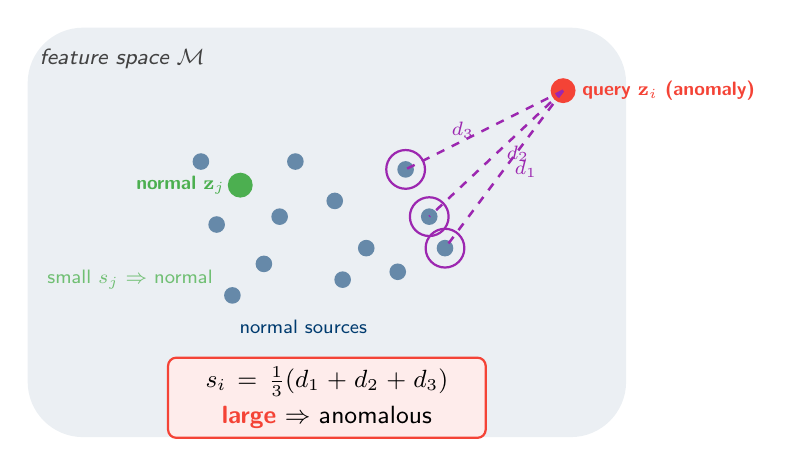
\begin{tikzpicture}

  % Feature space background
  \fill[uwcblue!8, rounded corners=20pt]
    (-3.8,-2.6) rectangle (3.8, 2.6);
  \node[font=\footnotesize\sffamily\itshape, text=darkgray]
    at (-2.6, 2.2) {feature space $\mathcal{M}$};

  % Normal cluster
  \foreach \x/\y in {
      -1.1/0.6, -0.6/0.2, -1.4/0.1, -0.8/-0.4,
      -1.2/-0.8, -0.4/0.9, -1.6/0.9,
       0.1/0.4,  0.5/-0.2, 0.2/-0.6,
       1.0/0.8,  1.3/0.2,  0.9/-0.5, 1.5/-0.2}
    \fill[uwcblue!60] (\x,\y) circle (3pt);
  \node[font=\scriptsize\sffamily, text=uwcblue] at (-0.3,-1.2)
    {normal sources};

  % Anomaly point
  \fill[scorecol] (3.0, 1.8) circle (4.5pt);
  \node[font=\scriptsize\sffamily\bfseries, text=scorecol,
        right=2pt] at (3.05, 1.8) {query $\mathbf{z}_i$ (anomaly)};

  % k=3 nearest neighbours
  \coordinate (A)  at (3.0, 1.8);
  \coordinate (N1) at (1.5,-0.2);
  \coordinate (N2) at (1.3, 0.2);
  \coordinate (N3) at (1.0, 0.8);

  \draw[knncolor, dashed, line width=0.9pt] (A) -- (N1)
    node[midway, right, font=\scriptsize\sffamily\color{knncolor}]{$d_1$};
  \draw[knncolor, dashed, line width=0.9pt] (A) -- (N2)
    node[midway, right, font=\scriptsize\sffamily\color{knncolor}]{$d_2$};
  \draw[knncolor, dashed, line width=0.9pt] (A) -- (N3)
    node[midway, left,  font=\scriptsize\sffamily\color{knncolor}]{$d_3$};

  \foreach \pt in {N1,N2,N3}
    \draw[knncolor, thick] (\pt) circle (7pt);

  % Score annotation box
  \node[draw=scorecol, fill=scorecol!10, rounded corners=3pt,
        font=\small\sffamily, line width=0.8pt,
        text width=3.8cm, align=center]
    at (0.0, -2.1)
    {$s_i = \frac{1}{3}(d_1 + d_2 + d_3)$\\[2pt]
     \textcolor{scorecol}{\textbf{large}} $\Rightarrow$ anomalous};

  % Normal example
  \fill[combinecol] (-1.1, 0.6) circle (4.5pt);
  \node[font=\scriptsize\sffamily\bfseries, text=combinecol,
        left=2pt] at (-1.1, 0.6) {normal $\mathbf{z}_j$};
  \node[font=\scriptsize\sffamily\color{combinecol!80}]
    at (-2.5,-0.6) {small $s_j \Rightarrow$ normal};

\end{tikzpicture}
\caption{%
  \textbf{$k$-NN anomaly scoring} ($k=3$).
  Normal objects (blue) cluster tightly in feature space; an anomalous
  query (red) lies far from all stored points.
  Its score $s_i$ is the mean of its three nearest-neighbour distances,
  which is large for anomalies and small for normal sources.}
\label{fig:scoring}
\end{figure}

%% ─────────────────────────────────────────────────────────────────────
\subsection{Layer Ablation}
\label{sec:patchcore:ablation}

To confirm that combining both layers improves over either alone, we run
a three-way ablation --- Layer~2 only (256\,dim), Layer~3 only (512\,dim),
and the concatenation (768\,dim) --- using the same $k$-NN scorer for all
variants.  \Cref{fig:ablation_diagram} illustrates the three conditions.

%% ─────────────────────────────────────────────────────────────────────
%%  FIGURE 3  Ablation illustration
%% ─────────────────────────────────────────────────────────────────────
\begin{figure}[H]
\centering
\begin{tikzpicture}[node distance=0.7cm]

  \node[font=\small\sffamily\bfseries, text=darkgray] (bblabel) at (0,0)
    {WideResNet50 (frozen)};

  \node[layerbox=layer2col, below left=0.6cm and 1.6cm of bblabel]
    (L2) {\textcolor{layer2col}{\textbf{Layer 2}}\\256-dim};
  \node[layerbox=layer3col, below right=0.6cm and 1.6cm of bblabel]
    (L3) {\textcolor{layer3col}{\textbf{Layer 3}}\\512-dim};

  \draw[arrow, uwcblue!50] (bblabel) -- (L2);
  \draw[arrow, uwcblue!50] (bblabel) -- (L3);

  % Variant A
  \node[block=2.5cm, below=1.0cm of L2] (varA)
    {\textbf{Variant A}\\Layer~2 only\\$k$-NN scorer};
  \draw[arrow] (L2) -- (varA);

  % Variant B
  \node[block=2.5cm, below=1.0cm of L3] (varB)
    {\textbf{Variant B}\\Layer~3 only\\$k$-NN scorer};
  \draw[arrow] (L3) -- (varB);

  % Variant C (combined)
  \node[highlight=3.0cm, below=2.2cm of bblabel] (varC)
    {\textbf{PatchCore (Combined)}\\Layer~2 $\oplus$ Layer~3\\$k$-NN scorer};
  \draw[arrow] (L2.south) -- ++(0,-0.4) -| (varC.north west);
  \draw[arrow] (L3.south) -- ++(0,-0.4) -| (varC.north east);

  % Performance labels
  \node[font=\scriptsize\sffamily, text=darkgray, below=0.3cm of varA]
    (perfA) {ROC-AUC$_{\rm A}$};
  \node[font=\scriptsize\sffamily, text=darkgray, below=0.3cm of varB]
    (perfB) {ROC-AUC$_{\rm B}$};
  \node[font=\scriptsize\sffamily\bfseries, text=combinecol,
        below=0.3cm of varC]
    (perfC) {ROC-AUC$_{\rm C}$ (target)};

  \draw[arrow, darkgray!50] (varA) -- (perfA);
  \draw[arrow, darkgray!50] (varB) -- (perfB);
  \draw[arrow, combinecol]  (varC) -- (perfC);

\end{tikzpicture}
\caption{%
  \textbf{Layer ablation design.}
  Three variants use the same $k$-NN scorer but differ in feature input.
  Variant~A uses only local Layer~2 features (256-dim);
  Variant~B uses only semantic Layer~3 features (512-dim);
  the combined PatchCore model concatenates both (768-dim).
  Comparing ROC-AUC values isolates the marginal value of each layer.}
\label{fig:ablation_diagram}
\end{figure}

%% ─────────────────────────────────────────────────────────────────────
\subsection{Component Decomposition: PatchCore vs.\ $k$-NN}
\label{sec:patchcore:decomp}

The final anomaly score arises from the interaction of \emph{two
components}: the feature extractor (PatchCore backbone) and the anomaly
scorer ($k$-NN distance).  To quantify each component's contribution we
design a $2\times2$ ablation (\Cref{fig:2x2}).

%% ─────────────────────────────────────────────────────────────────────
%%  FIGURE 4  2x2 component grid
%% ─────────────────────────────────────────────────────────────────────
\begin{figure}[H]
\centering
\begin{tikzpicture}

  % Column / row labels
  \node[font=\small\sffamily\bfseries, text=darkgray]
    at (2.0, 1.0) {BYOL features};
  \node[font=\small\sffamily\bfseries, text=uwcblue]
    at (5.4, 1.0) {PatchCore features};

  \node[font=\small\sffamily\bfseries, text=darkgray,
        rotate=90] at (-0.9, -0.7) {Centroid scorer};
  \node[font=\small\sffamily\bfseries, text=knncolor,
        rotate=90] at (-0.9, -3.2) {$k$-NN scorer};

  % Cell D (floor)
  \node[block=3.0cm, fill=lightgray] (D) at (2.0,-0.7)
    {\textbf{(D)}\\BYOL + centroid\\\textit{floor}};

  % Cell C
  \node[block=3.0cm, fill=combinecol!10, draw=combinecol] (C) at (5.4,-0.7)
    {\textbf{(C)}\\PatchCore + centroid\\feature effect only};

  % Cell B
  \node[block=3.0cm, fill=knncolor!10, draw=knncolor] (B) at (2.0,-3.2)
    {\textbf{(B)}\\BYOL + $k$-NN\\$k$-NN effect only};

  % Cell A (full system)
  \node[highlight=3.0cm, fill=uwcgold!20, draw=uwcgold] (A) at (5.4,-3.2)
    {\textbf{(A)} $\leftarrow$ Full system\\PatchCore + $k$-NN\\\textit{target}};

  % Gain arrows
  \draw[{Latex[length=2.5mm]}-{Latex[length=2.5mm]},
        combinecol, thick, dashed]
    (D.east) -- (C.west)
    node[midway, above, font=\scriptsize\sffamily\color{combinecol}]
      {feature gain $\Delta_\text{feat}$};

  \draw[{Latex[length=2.5mm]}-{Latex[length=2.5mm]},
        knncolor, thick, dashed]
    (D.south) -- (B.north)
    node[midway, left=2pt, font=\scriptsize\sffamily\color{knncolor}]
      {$k$-NN gain $\Delta_{k\text{-NN}}$};

  \draw[{Latex[length=2.5mm]}-{Latex[length=2.5mm]},
        uwcgold!80!black, thick]
    (D.south east) -- (A.north west)
    node[midway, below right=1pt,
         font=\scriptsize\sffamily\color{uwcgold!80!black}]
      {total gain};

  % Equation box
  \node[draw=darkgray!40, fill=lightgray, rounded corners=3pt,
        text width=7.0cm, font=\scriptsize\sffamily, align=left,
        line width=0.5pt]
  at (3.7, -5.2) {
    $\Delta_\text{feat} = \mathrm{AUC}(A) - \mathrm{AUC}(B)$
      \hfill same scorer, better features\\[3pt]
    $\Delta_{k\text{-NN}} = \mathrm{AUC}(A) - \mathrm{AUC}(C)$
      \hfill same features, better scorer\\[3pt]
    $\Delta_\text{int} = [\mathrm{AUC}(A){-}\mathrm{AUC}(D)]
      - \Delta_\text{feat} - \Delta_{k\text{-NN}}$
      \hfill interaction
  };

\end{tikzpicture}
\caption{%
  \textbf{$2\times2$ component decomposition.}
  Two feature choices (BYOL vs.\ PatchCore) crossed with two scoring
  strategies (centroid distance vs.\ $k$-NN) yield four conditions A--D.
  Performance differences between conditions isolate the marginal
  contribution of each component and any synergistic interaction.}
\label{fig:2x2}
\end{figure}

The three quantities are defined as:
\begin{align}
  \Delta_\text{feat}
    &= \mathrm{AUC}(A) - \mathrm{AUC}(B)
    && \text{PatchCore features over BYOL, scorer fixed}
    \label{eq:feat_gain}\\
  \Delta_{k\text{-NN}}
    &= \mathrm{AUC}(A) - \mathrm{AUC}(C)
    && \text{$k$-NN over centroid, PatchCore features fixed}
    \label{eq:knn_gain}\\
  \Delta_\text{int}
    &= \bigl[\mathrm{AUC}(A){-}\mathrm{AUC}(D)\bigr]
       - \Delta_\text{feat} - \Delta_{k\text{-NN}}
    && \text{interaction / synergy}
    \label{eq:interaction}
\end{align}
A positive $\Delta_\text{int}$ indicates that the two components
\emph{amplify} each other beyond their individual contributions; a
negative value indicates redundancy.

%% ─────────────────────────────────────────────────────────────────────
\subsection{Evaluation Protocol}
\label{sec:patchcore:eval}

Evaluation follows the same four-metric protocol used throughout this
work (\Cref{tab:metrics}).  All scores are computed on the intersection
of catalogue objects that have both a human label and an extracted
image feature vector.

\begin{table}[H]
\centering
\caption{Evaluation metrics.  $\hat{s}_i$ is the predicted anomaly
  score; $y_i \in \{0,1\}$ is the binary label ($y_i=1$ if human
  score $\geq 4$).}
\label{tab:metrics}
\smallskip
\begin{tabular}{lp{7.5cm}}
\toprule
\textbf{Metric} & \textbf{Definition} \\
\midrule
ROC-AUC
  & Area under the receiver operating characteristic curve;
    threshold-free, insensitive to class imbalance. \\
PR-AUC
  & Area under the precision--recall curve; sensitive to
    performance on the (rare) positive class. \\
Recall@100
  & Fraction of true anomalies (score $\geq 4$) recovered
    in the top-100 ranked candidates. \\
Spearman $\rho$
  & Rank correlation between $\hat{s}_i$ and the raw human
    score $\in\{1,\ldots,5\}$; measures calibration across
    the full severity spectrum. \\
\bottomrule
\end{tabular}
\end{table}

The Protege baseline (PCA-based active learning with human labels) is
included in every comparison as the reference ceiling, since it has
access to human feedback that PatchCore deliberately avoids.

%% ─────────────────────────────────────────────────────────────────────
\subsection{Implementation Notes}
\label{sec:patchcore:impl}

All experiments are implemented in PyTorch~\citep{Paszke2019} using the
\texttt{torchvision.models.wide\_resnet50\_2} backbone with
\texttt{IMAGENET1K\_V1} weights.  Distance computation uses
\texttt{sklearn.metrics.pairwise\_distances\_chunked} with
\texttt{working\_memory=256\,MB} to avoid materialising the full
$N\times N$ distance matrix.  Extracted features are cached to a Parquet
file so the expensive extraction pass runs only once.
All code is contained in the accompanying notebook
\texttt{patchcore\_extraction.ipynb}.

%% ─────────────────────────────────────────────────────────────────────
%%  BibTeX entries — add these to your .bib file
%% ─────────────────────────────────────────────────────────────────────
%
% @inproceedings{Roth2022,
%   author    = {Karsten Roth and Latha Pemula and Joaquin Zepeda and
%                Bernhard Sch{\"o}lkopf and Thomas Brox and Peter Gehler},
%   title     = {Towards Total Recall in Industrial Anomaly Detection},
%   booktitle = {Proceedings of the IEEE/CVF CVPR},
%   year      = {2022},
%   pages     = {14318--14328},
% }
%
% @inproceedings{Zagoruyko2016,
%   author    = {Sergey Zagoruyko and Nikos Komodakis},
%   title     = {Wide Residual Networks},
%   booktitle = {British Machine Vision Conference (BMVC)},
%   year      = {2016},
% }
%
% @inproceedings{Paszke2019,
%   author    = {Adam Paszke and others},
%   title     = {{PyTorch}: An Imperative Style, High-Performance
%                Deep Learning Library},
%   booktitle = {Advances in Neural Information Processing Systems},
%   volume    = {32},
%   year      = {2019},
% }
